\section{Radio definida por Software}

Software Defined Radio (SDR) es un sistema de comunicación en el que parte del procesamiento de señales analógicas tradicionalmente realizado mediante circuitos electrónicos analógicos se reemplaza por el procesamiento de señales digitales (DSP) y cualquier tipo de computadora o sistema integrado que ejecute el software DSP.

Al reemplazar los componentes de hardware con procesamiento de señales, insertando ADC/DAC lo más arriba posible del flujo de señal y procesar la señal digital, se pueden utilizar sistemas muy flexibles y de propósito general. 

Idealmente, colocando un ADC o DAC directamente en la antena se obtendría la máxima flexibilidad, pero esto no es práctico y los sistemas SDR suelen incluir un frontend de  radiofrecuencia (RF) antes muestrear como en el diagrama conceptual. 

A continuación que representa el sistema típico de SDR:

\begin{figure}[h!]
\centering

\includegraphics[width=0.8\textwidth]{fig/SDR.png}
\caption{Diagrama ejemplo de un sistema SDR.}
\label{fig:frontend}
\end{figure}

Hay muchos SDR de propósitos generales disponibles en el mercado electrónico. 
Una opción económica para receptores son los dongles USB con sintonizador de TV DVB-T basados en el chipset RTL2832U. Estos dongles están diseñados para recibir TV DVB-T, pero los controladores de Osmocom pueden convertirlos en receptores SDR de banda ancha y se conoce generalmente como RTL-SDR.

El dongle USB DVB-T genérico fue modificado por NooElec para usarlo como SDR. 
Puede ver en la imagen el control remoto que viene con él para su uso original como sintonizador de TV. Tiene un conector de antena MCX estándar y viene con una pequeña antena de látigo.

\subsection{Arquitectura de los dongles USB para TV DVB-T basados en RTL2832U.}

La arquitectura general de los dongles RTL-SDR se basa en un receptor superheterodino que es un diseño popular para los receptores que deben poder procesar señales en una amplia gama de frecuencias seleccionadas por el usuario, aislando a partir de otras señales y amplificarlas. 


En los dongles RTL-SDR, la señal se muestrea a una frecuencia intermedia baja después de una etapa de filtrado y amplificación analógica y se procesa digitalmente. Los dongles RTL-SDR contienen 2 circuitos integrados importantes que implementan las diferentes funciones del receptor superheterodino:
\begin{itemize}
    \item Sintonizador: el extremo frontal de RF que implementa la parte de procesamiento de señal analógica del receptor y es responsable de la conversión descendente en la frecuencia intermedia.
    \item El RTL2832Utoma:muestras de la señal y realiza tareas adicionales de procesamiento de señales digitales, como la decimación. También maneja control USB. 
\end{itemize}

En las siguientes secciones se detallará la función de cada uno de estos componentes importantes. 



\subsection{FrontEnd Sintonizador.}

Existen dos familias principales de chips de sintonizador de interés para las aplicaciones de SDR, el ahora descontinuado Elonics E4000 y el sintonizador de radio Raphael Micro R820T / R820T2, que será el tema central de esta discusión. Las diferencias entre la T y la T2 son pequeñas, esencialmente equivalentes a una sensibilidad ligeramente mejor para propósitos prácticos.


\begin{figure}[h!]
\centering
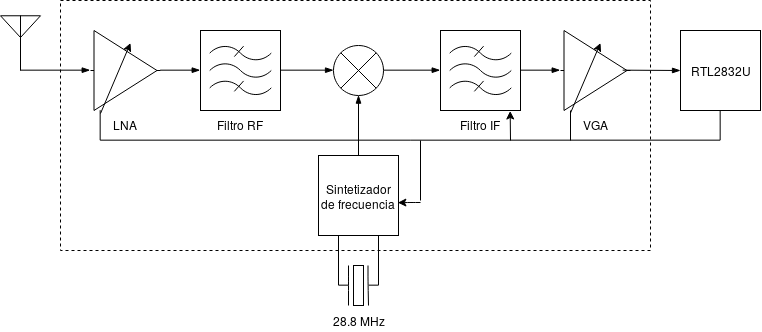
\includegraphics[width=0.8\textwidth]{fig/FrontendSDR.png}
\caption{Frontend}
\label{fig:frontend}
\end{figure}

La hoja de datos del R820T se filtró en línea, por lo que se sabe mucho sobre el funcionamiento interno de este chip. También una descripción de registro está disponible para el R820T2 que detalla los parámetros del sintonizador que se pueden configurar desde el exterior. A continuación se muestra un diagrama simplificado de alto nivel basado en el que se encuentra en la hoja de datos:

La señal que proviene del conector de la antena primero pasa por un amplificador de bajo ruido (LNA) y luego se filtra mediante un filtro pasa banda y un filtro de rechazo de imagen. 
Según la hoja de datos, el rechazo de la imagen es de 65 dBc.


\begin{table}[]
\begin{tabular}{|l|l|}
\hline

Tuner              &	Frequency range \\ \hline
Elonics E4000      &	\SI{52}{} a \SI{1100}{MHz}   \\ \hline
Rafael Micro R820T &	\SI{24}{} - \SI{1766}{MHz}  \\ \hline
Rafael Micro R828D &    \SI{24}{} - \SI{1766}{MHz}  \\ \hline
Fitipower FC0013   &	\SI{22}{} - \SI{1100}{MHz} \footnote{FC0013B/C, FC0013G has a separate L-band input, which is unconnected on most sticks} \\ \hline
Fitipower FC0012   &	\SI{22}{} - \SI{948.6}{MHz}  \\ \hline
FCI FC2580 	       &    \SI{146} - \SI{308}{MHz}  y \SI{438}{} - \SI{924}{MHz} \\ \hline

\end{tabular}
\end{table}

Un sintetizador de frecuencia basado en PLL fraccional genera el LO que se mezcla con esta señal filtrada para convertirlo a una frecuencia intermedia baja. 
El usuario controla la frecuencia del oscilador local directamente a través de los parámetros del sintetizador de frecuencia. 
Esto establece de manera indirecta la frecuencia de FI y si se usa inyección de lado alto o bajo. 
Los valores típicos para el IF de los dongles R820T son \SI{3.57}{MHz} y \SI{4.57}{MHz}, pero esencialmente depende de la implementación del controlador elegir qué valores usar (sujeto a los límites impuestos por los parámetros del sintetizador y el filtro de IF). 
El rango de frecuencia que el RTL-SDR puede sintonizar está determinado por el rango de frecuencias que puede generar el sintetizador de frecuencia dentro del chip. 
El rango oficial del R820T encontrado en la hoja de datos es de \SI{42}{} a \SI{1002}{MHz} con una resolución de sintonización de \SI{1}{Hz}, pero el rango real generalmente acordado es [24; 1766] MHz según lo determinado por la comunidad RTL-SDR. 
De hecho, utilizando un conjunto experimental de controladores, este rango de frecuencia se ha extendido hasta \SI{13}{} a \SI{1864}{MHz} con el límite superior que tiene cierta variabilidad.

Finalmente, una vez en la frecuencia intermedia, la señal se filtra de nuevo y pasa por un amplificador de ganancia variable (VGA). El filtro de IF suele ser más selectivo que el RF, ya que ese es el punto de las arquitecturas superheterodinas. En el caso del R820T, está compuesto por un filtro de paso bajo y uno de paso alto que puede configurarse para tener un ancho de banda tan bajo como \SI{300}{kHz}.

Sin embargo, sus valores estándar son \SI{6}{}, \SI{7}{} u \SI{8}{MHz}, ya que estos son los anchos de banda utilizados por las señales DVB-T. 
Hay 3 ganancias generales en el sintonizador que pueden controlarse a través de la configuración externa: el LNA, el mezclador y el VGA. 
Estas ganancias se pueden establecer manualmente, aunque sus valores precisos están ausentes de la hoja de datos. 
También se pueden configurar automáticamente a través del control automático de ganancia (AGC) para optimizar la relación señal a ruido (SNR). 
El LNA y el mezclador tienen un detector de potencia en sus salidas que se utiliza para controlar sus ganancias respectivas para este propósito. 
El VGA AGC se controla a través de un puerto de entrada analógica al sintonizador que está conectado a un detector de alimentación en el RTL2832U.
Una nota en los chips E4000 es que estos utilizan un IF de 0 Hz, por lo que en realidad no están implementando receptores superheterodinos. Esto tiene una consecuencia notable de producir un pico de CC a 0 Hz.

\subsection{RTL2832U}

Este es el IC que da el nombre al dongle RTL-SDR. A diferencia del sintonizador, las hojas de datos no están disponibles gratuitamente en línea. 
Por lo tanto, mucho de lo que se sabe sobre el funcionamiento interno de este chip ha sido resuelto por la comunidad RTL-SDR a través de ingeniería inversa. 

La descripción de Realtek del RTL2832U establece que el chip está diseñado como un demodulador DVB-T de alto rendimiento (con soporte adicional para FM y radio DAB). Como tal, incluye un ADC para muestrear la señal de IF proveniente de un sintonizador apropiado, todo el DSP especializado requerido para demodular DVB-T y un controlador USB compatible con una interfaz USB 2.0. El uso como SDR aprovecha el modo de "depuración" en el chip para entregar las muestras de representación de banda base digital compleja directamente a través de USB.
El siguiente diagrama en bloques representa las funciones que realiza el RTL2832U cuando se usa un IF que no es cero:
  
\begin{figure}[h!]
\centering
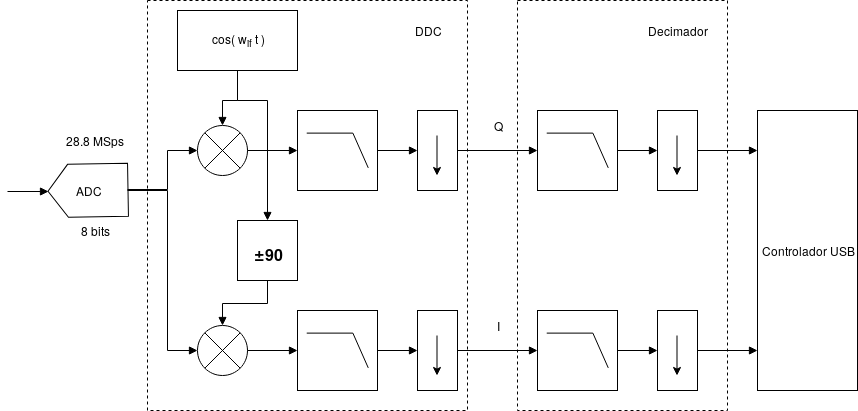
\includegraphics[width=0.8\textwidth]{fig/RTL2832U.png}
\caption{Frontend}
\label{fig:frontend}
\end{figure}

Inicialmente, la señal que sale del sintonizador se muestrea mediante un ADC de 8 bits que funciona a 28,8 MHz. No debe ocurrir un aliasing significativo para los valores bajos de IF admitidos si el filtro de IF es lo suficientemente selectivo como para eliminar cualquier señal fuerte fuera de su ancho de banda.
Un convertidor descendente digital (DDC) es responsable de convertir la señal digital a banda base compleja. El proceso de obtención de la representación de banda base compleja es similar al caso de tiempo continuo: la mezcla con una sinusoide compleja desplazará circularmente el espectro de IF a banda base. Luego, la señal puede filtrarse por un paso bajo y extraerse el muestreo para eliminar la parte innecesaria del espectro que se cambió a frecuencias más altas, ya que la señal de interés ahora está limitada por la banda por una frecuencia más baja. Los parámetros de configuración externa informan al DDC de la frecuencia IF y si el espectro está invertido (es decir, si el sintonizador es una inyección de lado alto).
Finalmente, se aplica la reducción (utilizando un filtro de paso bajo FIR y un submuestreo) para reducir la frecuencia de muestreo de la señal a un valor en el rango (225001, 300000) Hz o (900001, 3200000) Hz. Sin embargo, 2,56 MHz es la frecuencia de muestreo segura más alta generalmente acordada donde el chip no deja caer ninguna muestra (el USB aún puede dejarla caer). Esta decimación es lo que generalmente establece el límite superior en el ancho de banda de la señal muestreada (a menos que el ancho de banda del filtro IF se elija específicamente como más bajo que la frecuencia de Nyquist para la frecuencia de muestreo).
Las muestras de banda base complejas I y Q se envían a través de USB como enteros sin signo de 8 bits entrelazados.
   1. Un modelo de comportamiento de alto nivel
A veces es útil tener una imagen simplificada en mente de las partes internas de la RTL-SDR. Esta imagen, aunque no es perfectamente precisa, captura el comportamiento esencial del hardware al tiempo que oculta parte de la complejidad. A continuación se presenta uno de estos modelos de nivel de comportamiento de RTL-SDR, basado en el Laboratorio 6 delde curso de Sistemas de comunicación analógicos y digitalesStanford 2014:
   
En su esencia, el RTL-SDR nos proporciona una representación de banda de base compleja digital de la señal en cualquier banda de frecuencia con la que sintonizamos. Eliminando la complejidad añadida de la arquitectura superheterodina, el funcionamiento del RTL-SDR puede reducirse a:


Amplificación; 
* Encontrar la representación de banda base compleja mediante la mezcla con un sinusoide complejo y un filtro de paso bajo; 
* Muestreo. 
Estos son los pasos esenciales representados en el diagrama. Los tres parámetros esenciales que podemos variar son: los
* valores de ganancia (y el posible AGC); 
* La frecuencia central a la que estamos sintonizando; 
* La frecuencia de muestreo que puede llegar hasta ~ 2.56 MHz sin dejar caer muestras; 
* El ancho de banda del filtro que se puede elegir desde 300 kHz (haciendo uso del filtro IF dentro del sintonizador) hasta aproximadamente la frecuencia de Nyquist de la frecuencia de muestreo elegida (donde el factor limitante generalmente será el filtro de reducción dentro del RTL2832U) .